\documentclass[journal]{IEEEtai}
\usepackage[T1]{fontenc}
\usepackage{amsmath,amssymb}
\usepackage{graphicx,array,booktabs,tabularx}
\usepackage[colorlinks,urlcolor=blue,linkcolor=blue,citecolor=blue]{hyperref}
\usepackage{url}
\newcolumntype{Y}{>{\raggedright\arraybackslash}X}
\newcommand{\pct}{\%}
\newcommand{\R}{\mathbb{R}}
\setcounter{page}{1}
\begin{document}
\title{Violence and Goon Detection in a Crowd or Protest}
\author{Sudhakar Mishra, Vishal Gautam, Ishat Shivhare, Parth Parmar, Hanmant Jajulwar, Tanu Meena, and \mbox{Prakriti Manhar}
\thanks{The authors are with the Department of Artificial Intelligence, Sardar Vallabhbhai National Institute of Technology, Surat, India.}
\thanks{E-mail: sudhakarm@aid.svnit.ac.in; student addresses are \{u23ai127, u23ai071, u23ai084, u23ai098, u23ai076, u23ai114\}@coed.svnit.ac.in, respectively.}}
\markboth{}{}
\maketitle
\begin{abstract}
Violence classification in crowded video is difficult because nonviolent motion can resemble aggression and occlusion can degrade body-pose estimates. This study evaluates joint-reliability channels and nearest-person interaction features in a shared temporal convolutional classifier, alongside pretrained video references and limited video fine-tuning. Five custom source-grouped folds and three training seeds cover 245 unique crowd clips from 204 known source groups. Corrected pose centering yields mean accuracies of 77.0\%, 78.1\%, 78.6\%, and 74.7\% for baseline, reliability, interaction, and combined variants. A quality-only linear control reaches 77.6\%, and a matched detection-only temporal control reaches 72.5\%, indicating predictive detection cues. A frozen video encoder with logistic classifiers reaches 91.0\% mean crowd accuracy. On a separate supervised surveillance experiment, validation selects limited fine-tuning at epoch two and a threshold of 0.23. Fixed evaluation reduces missed fights from 43 to 25 but increases false alarms from 21 to 40, while accuracy changes from 84.0\% to 83.75\%. On 1,000 external hockey clips, frozen and fine-tuned video accuracy is 70.8\% and 81.1\%, whereas crowd-pose accuracy is 40.9\%. These exploratory results support modest pose-feature gains, substantial detection-cue signal, and a tradeoff between recall and false alarms. Previously inspected footage, incomplete source audits, and pending independent label review limit confirmatory interpretation.
\end{abstract}
\begin{IEEEImpStatement}
This study supports transparent evaluation of violence classifiers by reporting errors, source-grouped comparisons, and the information retained by diagnostic controls. The results show why a high classification score cannot establish reliable incident detection: a model can miss fights, flag nonviolent clips, and transfer poorly across recording domains. Pose features reduce the representation of appearance but do not by themselves establish privacy protection or remove dataset bias. The implementation and saved experimental records can support reproducible classroom research and further independent evaluation. Operational use would require fresh reviewed footage, application-specific error analysis, and validation of temporal and deployment behavior. The current outputs classify whole clips and do not identify responsible people or infer intent.
\end{IEEEImpStatement}
\begin{IEEEkeywords}
Crowd video, domain transfer, human pose, input controls, temporal convolution, violence classification.
\end{IEEEkeywords}
\section{Introduction}
\IEEEPARstart{V}{ideo} violence classification asks whether a short sequence contains violent activity. The problem is difficult when several people overlap, when a camera moves, or when nonviolent activity contains rapid motion and close physical proximity. A cheering crowd can produce strong image motion, while an aggressive interaction can occupy only a small part of a frame. A clip classifier must therefore separate the label-relevant signal from recording conditions, detection behavior, and unrelated activity.

Motion descriptors and learned video representations provide established approaches to this problem \cite{hassner2012,nievas2011,serrano2015,cheng2020}. Human-pose representations offer a complementary description in terms of joints and trajectories. They can suppress some appearance information, but they introduce estimation errors, missing observations, and association decisions. A confidence channel may help distinguish reliable from unreliable joints, yet the same channel can also expose properties of the scene or recording domain. Relative-person geometry may describe interaction, but perspective and tracking errors can distort that geometry. These additions require evaluation rather than an assumed benefit.

The primary question of this study is whether explicit pose reliability and nearest-person interactions improve a fixed temporal baseline on crowd videos. We implement four feature variants using the same pose caches, source assignments, encoder family, and training budget. We also examine a correction to body centering, which otherwise changes abruptly when hip joints become unavailable. Matched fits compare the original fallback with a continuous offset estimate. The correction addresses feature construction and is distinct from a claim of improved external generalization.

A second question concerns the information that makes these classifiers effective. A seven-variable detection-quality classifier, a motion reference, a coverage ablation, and matched input controls test different aspects of the available signal. In particular, zeroing kinematic channels leaves confidence, validity, observation masks, neighbor counts, and coverage accessible. Shuffling derived slices disrupts their order but retains velocities already calculated from adjacent observations. These distinctions determine what conclusions the controls can support.

The study then adds a frozen pretrained video reference on the same crowd folds and a separate supervised experiment on RWF-2000. The latter fits a new classifier using the surveillance training release and develops one limited fine-tuning candidate. Validation alone selects its checkpoint and threshold. A fixed external Hockey Fight experiment compares that candidate, the original frozen surveillance reference, and a crowd-trained pose checkpoint. This follow-up tests recording-domain transfer and the consequences of changing the operating point, while preserving the original pose question.

The contributions are empirical and implementation-focused. First, we document a reproducible multi-person pose pipeline with confidence and nearest-person variants and a matched correction of the coordinate origin. Second, we report controlled evidence that detection-related inputs remain predictive and explain why an ordering control does not remove motion. Third, we provide separate crowd and surveillance video references and a validation-selected fine-tuning comparison with explicit miss and false-alarm counts. Finally, we connect aggregate results to decoded diagnostic videos, runtime measurements, and saved evaluation records.

The resulting evidence is mixed. Interaction features give the highest mean accuracy among the four corrected pose variants, but the combined variant performs worse than the baseline. The quality-only control is competitive, and frozen video features give a stronger crowd reference. Fine-tuning improves Fight recall on the surveillance evaluation, while slightly reducing accuracy and increasing false alarms. External pose transfer is poor. These findings describe the implemented models and experimental conditions, without establishing a novel general-purpose architecture or a deployment-ready detector.

The manuscript treats the evaluations as exploratory. Existing crowd and RWF footage had been inspected during earlier development, known source links do not exhaust all possible overlap, and independent label review remains pending. We retain those qualifications throughout the methods and results. The task is whole-clip binary classification. The outputs do not estimate the exact onset of violence, attribute responsibility to a person, or validate performance on an uninterrupted surveillance stream.

\section{Related Work}
\subsection{Violence datasets and motion representations}
Nievas et al. introduced video violence detection experiments and hockey fight footage as a benchmark \cite{nievas2011}. Hassner et al. studied violent crowd behavior using changes in optical-flow magnitude and provided the Violent-Flows dataset with classification and outbreak-detection protocols \cite{hassner2012}. Serrano Gracia et al. also examined efficient fight detection using motion information \cite{serrano2015}. These studies establish that motion is useful, while the recording context and prediction target determine how a reported result should be interpreted.

RWF-2000 provides a surveillance-oriented collection and a Flow Gated Network combining three-dimensional convolution and optical-flow information \cite{cheng2020}. We use its released footage for a separate supervised video reference. Our frozen R3D-18 classifier and limited fine-tuning are not a reproduction of the published Flow Gated Network. Differences in architecture, preprocessing, source exclusions, and development history prevent a direct benchmark superiority claim. Similarly, we retain custom source-grouped crowd folds instead of presenting them as the supplied Violent-Flows protocol.

\subsection{Skeleton sequence modeling}
Spatial Temporal Graph Convolutional Networks learn spatial and temporal patterns on skeleton graphs \cite{yan2018}. Two-stream adaptive graph convolution further learns graph structure and combines different skeleton signals \cite{shi2019}. These methods demonstrate that skeleton-based action recognition and learned body relationships predate this study. Our temporal convolutional encoder is intentionally small and uses shared per-person processing followed by masked set pooling. It does not implement a graph-convolution architecture or establish that simple nearest-neighbor features replace learned graph reasoning.

Famouri et al. combine pose sequences with temporal classification and federated learning for surveillance anomaly detection \cite{famouri2025}. Their work motivates evaluating skeleton sequences in surveillance, but its anomaly labels, learning setup, and representation differ from ours. Hegiste et al. study pose-based federated recognition of industrial worker gestures \cite{hegiste2025}. That application provides pose-processing context rather than evidence of violence classification performance. We implement neither federated training nor formal privacy mechanisms. Removing raw appearance from classifier input alone does not certify anonymity or privacy.

Temporal convolution is also an established sequence-modeling approach. Bai et al. systematically compare generic convolutional and recurrent models across sequence tasks \cite{bai2018}. We use residual dilated convolutions as a practical baseline, with masking for absent person observations. The classifier operates on complete clips with symmetric temporal padding. Its implementation does not assume a causal or streaming inference setting.

\subsection{Pretrained video representations}
Tran et al. compare spatiotemporal convolution families for action recognition \cite{tran2018}. The R3D-18 implementation available in TorchVision supplies a pretrained three-dimensional residual encoder \cite{torchvision}. Its Kinetics-400 pretraining comes from a broad human-action dataset \cite{kay2017}. A frozen encoder allows a small downstream classifier to exploit that representation without fitting all encoder parameters on a limited crowd corpus. Limited fine-tuning can then adapt later layers, but its usefulness must be assessed using a fixed selection boundary.

This study separates three uses of video features: crowd-trained logistic classifiers on frozen embeddings, a new RWF-trained logistic classifier, and a layer4 fine-tuning candidate initialized from the supervised reference. These models share an encoder family but differ in training data and learned parameters. Their accuracies therefore cannot be treated as successive scores on a single unchanged task. We compare models within their specified evaluation partitions and use external scores only after sealing model and threshold choices.

\subsection{Position of the present study}
Our emphasis is on controlled diagnosis rather than a claim that reliability channels, skeleton interactions, or pretrained video features are new. The experiments ask which additions help a fixed implementation, which information remains after an ablation, and how a selected video candidate changes errors. Independent label correctness, complete source separation, and pretraining overlap are separate questions. Artifact reproduction supports consistency of saved computation; it does not answer those questions automatically.

Table~\ref{tab:related} summarizes the relationship between the main foundations and the implemented task. Published task scores are deliberately omitted because their protocols and model families differ from this study.
\begin{table*}[t]
\caption{Foundation studies and their relationship to this implementation. These are methodological references, not matched performance comparisons.}
\label{tab:related}\centering
\begin{tabularx}{\textwidth}{lYY}
\toprule
Reference & Relevant idea or resource & Difference from the present study\\
\midrule
Nievas et al. \cite{nievas2011} & Video fight classification and hockey footage & Hockey is an external fixed-score domain here.\\
Hassner et al. \cite{hassner2012} & Crowd motion and Violent-Flows & We use custom source-grouped folds and whole-clip outputs.\\
Cheng et al. \cite{cheng2020} & RWF-2000 and a video/flow network & We use frozen R3D-18 heads and limited layer4 adaptation.\\
Yan et al.; Shi et al. \cite{yan2018,shi2019} & Skeleton graph and temporal modeling & Our encoder is a per-person TCN with nearest-person descriptors.\\
Famouri et al. \cite{famouri2025} & Pose sequences for surveillance anomalies & We study binary violence and use centralized training.\\
Hegiste et al. \cite{hegiste2025} & Pose processing for worker actions & Industrial gestures do not validate crowd violence recognition.\\
Tran et al. \cite{tran2018} & Spatiotemporal residual video encoding & We evaluate a downstream pretrained reference and bounded fine-tuning.\\
\bottomrule
\end{tabularx}
\end{table*}

\section{Data and Evaluation Boundaries}
\subsection{Crowd corpus and source grouping}
The local Violent-Flows release contains 246 low-resolution AVI files, with 123 supplied labels in each class. Removing one byte-identical nonviolent duplicate leaves 245 unique files: 123 violent and 122 nonviolent clips. All retained clips are fully decoded before selecting frame indices. Container frame counts are recorded as metadata and checked against the decoded length, rather than treated as a reliable sampling denominator.

Filename-derived source keys provide an initial grouping. For crowd filenames, the grouping removes the search-category prefix and retains source-title, uploader, and identifier information. Prefix-compatible truncated identifiers are conservatively linked when the title and uploader also match. This rule addresses a development-stage finding that exact string keys could leave related clips in separate partitions. It does not establish that every shared recording has been detected.

Additional source triage examines shared visual content. All 245 clips were decoded, giving 22,027 frames. Densely sampled full-frame and central-crop evidence used perceptual hashes, grayscale correlation, and temporal alignment to screen pairs of different filename groups. The project inspected 20 candidate evidence sheets and recorded 13 supported source links, two of which were redundant through existing groups. The number of known groups decreased from 215 to 204. Shared recordings can include different segments or crops rather than byte-identical files. This source inspection retained the supplied violence labels and did not constitute independent label reannotation.

The repeated study assigns each complete known source group to one of five custom stratified folds. In each rotation, one fold supplies 49 test clips, the preceding fold supplies 49 validation clips, and the remaining folds supply 147 training clips. All clips appear once as test data per training seed. The three temporal-model seeds are 42, 123, and 2026. Each deterministic logistic control is fitted once per fold because repeating a deterministic fit under different seed labels would not provide additional training variation.

These assignments differ from the dataset's supplied fold protocol. Existing footage and preliminary outputs had already been examined during development. The repeated results therefore describe exploratory source-grouped evaluation, with residual uncertainty about unidentified related footage. They do not represent an untouched benchmark or a confirmatory test of a hypothesis chosen before all dataset inspection.

\subsection{Supervised surveillance partition}
RWF-2000 contains 2,000 released clips, balanced across Fight and NonFight \cite{cheng2020}. The local release has 1,600 training files and 400 files under the directory named \texttt{val}. We use the latter as the released evaluation partition. A separate validation split comes only from released training footage. This naming distinction is important: the 317 development-validation clips select models, while the 400 released evaluation clips provide fixed scores after selection.

Source identifiers are extracted without using the class directory. Byte-identical links merge source groups, including groups that contain both supplied labels. The first fold from five-way stratified group splitting with split seed 42 supplies validation, and the remaining groups supply training. The duplicate audit identifies six train/evaluation byte-duplicate pairs. Excluding all training clips in the linked evaluation source groups removes seven files. Five further same-label development duplicates are also excluded. The final partitions contain 1,271 training and 317 validation clips, while all 400 evaluation clips remain.

The training partition contains 633 NonFight and 638 Fight clips. Validation contains 158 NonFight and 159 Fight clips. Evaluation contains 200 clips per class. Known group counts are 603, 153, and 180 for training, validation, and evaluation, respectively. Table~\ref{tab:data} records the primary denominators. Filename and byte grouping do not exhaust near-duplicate detection. Moreover, all 400 released evaluation clips had been inspected and scored in earlier transfer experiments. Later validation-only selection limits direct evaluation-driven tuning, but it cannot undo that prior exposure.

\begin{table*}[t]
\caption{Datasets and primary evaluation partitions. Source counts refer to the project's known groups, not independently verified recording identities.}
\label{tab:data}\centering
\begin{tabularx}{\textwidth}{lrrrrY}
\toprule
Study & Train & Validation & Evaluation & Known groups & Protocol\\
\midrule
Crowd, each rotation & 147 & 49 & 49 & 204 total & Five custom grouped folds, three TCN seeds; 245 unique clips.\\
RWF supervised & 1,271 & 317 & 400 & 603/153/180 & Validation from training release; duplicate-linked train exclusions.\\
Hockey external & 0 & 0 & 1,000 & Unaudited & Fixed models, normalization, and thresholds; no external fitting.\\
\bottomrule
\end{tabularx}
\end{table*}

\subsection{External hockey corpus}
The external study uses the Hockey Fight mirror \cite{hockeymirror}, pinned to revision \texttt{2009e360f0887c9d0495f684a488519a625b0293}. Its 1,000 clips contain 500 supplied labels per class. The inventory has 997 unique byte hashes and three duplicate files. All released mirror files remain in the primary denominator, rather than silently removing duplicates after scoring. No byte-identical overlap was found against the compared 2,245-file crowd/RWF inventory.

That result establishes only the outcome of this byte comparison. It does not certify independent source games, identify temporal overlap, or rule out near-duplicates and pretraining overlap. Hockey broadcasts contain camera motion, editing, player equipment, and action patterns that differ from surveillance and crowd footage. We treat this corpus as a recording-domain stress test. Its supplied labels remain unchanged and independently unreviewed.

\subsection{Boundaries between fitting and scoring}
Every fitted classifier uses training-only normalization and training data for parameter estimation. Validation chooses checkpoints, logistic regularization when specified, and decision thresholds. The fine-tuning candidate must pass a recorded promotion rule before evaluation. The external protocol fixes all model paths, hashes, normalization, and thresholds before its scoring pass. No hockey result selects a new model or operating point.

The frozen RWF video reference remains the predeclared primary external model. Fine-tuned video results are supplementary, and the crowd-pose checkpoint is a transfer diagnostic. We retain these roles after seeing the results. The selected pose checkpoint is the corrected interactions model from fold 1, seed 42, with threshold 0.62, chosen by a fixed convention rather than by external accuracy. Its external score belongs to one saved checkpoint; it is distinct from the mean over all crowd folds and seeds.

Independent full-video label review is pending. The project prepared a neutral review pack, but no independent reviewer has completed it. Computational audits and author-side viewing do not substitute for that review. All findings use the supplied labels, and all primary metric denominators retain the declared clips, including cases with poor pose support.

\section{Pose Representation and Temporal Classifier}
\begin{figure*}[t]
\centering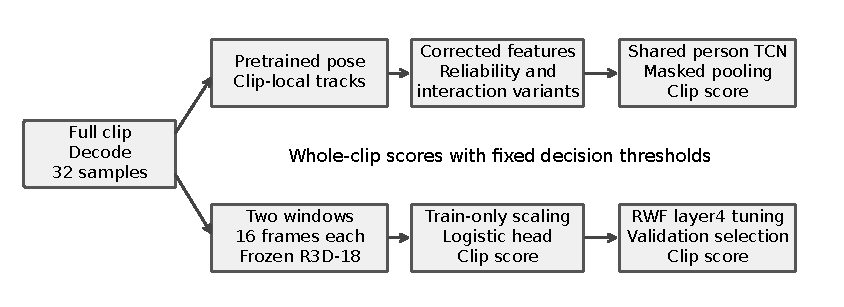
\includegraphics[width=\textwidth]{figures/pipeline.pdf}
\caption{Implemented representation paths. Pretrained estimators supply poses or video embeddings. Pose variants use a shared temporal encoder, while separate crowd and RWF logistic heads use frozen video features. Layer4 fine-tuning is a subsequent RWF development experiment. Each path produces a whole-clip score.}
\label{fig:pipeline}
\end{figure*}
\subsection{Sampling and pose estimation}
For a clip with $N$ decoded frames, we select $T=32$ indices uniformly across the complete sequence. Repeated indices are possible for clips shorter than $T$. Sampling timestamps use the selected indices and recorded frame rate, and velocity denominators have a small positive floor. The pretrained YOLO11n-pose estimator supplies normalized boxes and COCO-17 keypoints \cite{ultralytics}. Extraction uses image size 640, box confidence 0.2, joint-validity threshold 0.25, and at most 100 detections per sampled image. Estimator weights and settings are fixed for each recorded extraction signature.

Let $\mathbf{q}_{tpj}\in\R^2$ be the image-normalized coordinates of joint $j$ for track $p$ at sampled time $t$, and let $c_{tpj}$ be its confidence. Let $m_{tp}\in\{0,1\}$ denote an observed track. Joint validity is
\begin{equation}
v_{tpj}=m_{tp}\,\mathbf{1}[c_{tpj}\geq 0.25].
\label{eq:valid}
\end{equation}
Detector confidence expresses estimator output and is not a calibrated probability of joint correctness or violence. Missing detections do not establish absence of violent activity.

\subsection{Clip-local association and track packing}
Hungarian assignment \cite{kuhn1955} associates boxes within each clip using a cost combining intersection-over-union (IoU) and normalized center distance. A candidate link is permitted when IoU is at least 0.1 or center distance is at most 0.18. Its cost is $(1-\mathrm{IoU})+2d$, where $d$ is center distance. Tracks remain eligible through two missing sampled observations, and unmatched detections receive new identifiers. IDs reset at the beginning of each clip.

The pipeline retains $P=8$ tracks with the largest sum of observed keypoint-confidence signal. Empty slots contain zero values and an absent mask. The packed raw tensors have dimensions $T\times P\times17\times3$ for keypoints and $T\times P\times4$ for boxes. Association can fragment under occlusion, rapid movement, or a camera cut, and the eight-track limit can discard people. This implementation has no independently measured identity-switch rate or person-attribution accuracy.

\subsection{Continuous body origin}
Body normalization requires an origin. With both hip joints valid, the observed midpoint $\mathbf{h}_{tp}$ supplies that origin. Let $\mathbf{b}_{tp}$ be the box center. The legacy implementation switches directly to $\mathbf{b}_{tp}$ when a hip is missing. A change in the difference between hip and box centers can then appear as joint motion even if body motion is unchanged.

The corrected implementation estimates a continuous hip-to-box offset inside each uninterrupted observed track segment. At reliable hip anchors, the offset is $\mathbf{o}_{tp}=\mathbf{h}_{tp}-\mathbf{b}_{tp}$. Linear interpolation in sampled time fills offsets at missing-hip observations, with nearest-anchor extension at segment boundaries. For segments without reliable hip anchors, box center remains the fallback. The origin is
\begin{equation}
\mathbf{a}_{tp}=
\begin{cases}
\mathbf{h}_{tp}, & \text{both hips valid},\\
\mathbf{b}_{tp}+\widetilde{\mathbf{o}}_{tp}, & \text{anchors exist},\\
\mathbf{b}_{tp}, & \text{no hip anchor in segment}.
\end{cases}
\label{eq:center}
\end{equation}
Interpolation does not fill absent person observations. It uses the complete observed segment and is therefore an offline operation. Future anchors can influence an earlier missing-hip origin. The procedure uses no class labels, but it remains sensitive to box jitter, bad hip estimates, and association errors. The matched centering experiment fits all classifiers afresh for both schemas.

\subsection{Body coordinates and velocity}
Let $s_{tp}$ be the normalized box-diagonal length, floored at 0.03. We calculate body-centered coordinates
\begin{equation}
\mathbf{x}_{tpj}=v_{tpj}\,\operatorname{clip}
\left((\mathbf{q}_{tpj}-\mathbf{a}_{tp})/s_{tp},-3,3\right).
\end{equation}
Joint velocity uses actual sampled-time differences and only jointly valid neighboring observations:
\begin{equation}
\mathbf{u}_{tpj}=v_{tpj}v_{t-1,p,j}\,
\operatorname{clip}\left(
\frac{\mathbf{x}_{tpj}-\mathbf{x}_{t-1,p,j}}{\Delta t_t},-10,10\right),
\label{eq:velocity}
\end{equation}
where $\Delta t_t$ is floored at $10^{-3}$ s and the first velocity is zero. The baseline concatenates two coordinates and two velocity components for each of 17 joints, giving 68 channels per person and time.

The reliability variant multiplies positions and velocities by current joint confidence and appends 17 masked confidence channels and 17 validity channels. This yields 102 channels. The confidence weighting is a fixed feature operation rather than a learned uncertainty model. Validity information remains predictive even when a joint coordinate itself is unavailable.

\subsection{Nearest-person interaction features}
Interactions use shared image-normalized origins before individual scale normalization. For each observed person, the nearest other observed origin is selected by Euclidean distance. Let its offset be $\mathbf{r}_{tp}$ and its relative origin velocity be $\dot{\mathbf{r}}_{tp}$. The eight interaction channels are distance, two offset components, two relative-velocity components, signed radial relative velocity, normalized neighbor count, and neighbor presence. Radial relative velocity is
\begin{equation}
\gamma_{tp}=\operatorname{clip}
\left(\frac{\mathbf{r}_{tp}^{\mathsf T}\dot{\mathbf{r}}_{tp}}
{\max(\|\mathbf{r}_{tp}\|,10^{-4})},-10,10\right).
\end{equation}
Each origin velocity is the sampled-time difference of that person's image-normalized origin, clipped componentwise to $[-10,10]$ and set to zero unless that person is observed at both adjacent samples. The relative velocity subtracts the current person's origin velocity from the selected neighbor's origin velocity. It is not obtained by differentiating the nearest-neighbor offset across possible neighbor changes. Negative radial velocity indicates approach under this offset convention. Neighbor count divides the number of other observed people by $P-1$. The interaction-only variant has 76 channels, and the combined reliability/interaction variant has 110. When no neighbor is observed, the interaction vector is zero.

These descriptors use two-dimensional apparent geometry. Perspective means that image distance is not physical separation, and the nearest visible origin need not be the person participating in an interaction. Camera motion affects origin velocity. We therefore describe these as candidate interaction cues and do not interpret them as reliable contact, intent, or aggressor measurements.

\begin{table}[t]
\caption{Pose feature variants. Parameter counts use the shared 48-channel temporal encoder and coverage-enabled classifier.}
\label{tab:variants}\centering
\begin{tabular}{lrr}
\toprule Variant & Input channels & Parameters\\
\midrule Baseline & 68 & 36,001\\
Reliability & 102 & 37,633\\
Interactions & 76 & 36,385\\
Combined & 110 & 38,017\\
\bottomrule
\end{tabular}
\end{table}

\subsection{Temporal encoding and person pooling}
The classifier shares one temporal encoder across person slots. A $1\times1$ convolution projects each person's feature sequence to 48 hidden channels. Three residual blocks use temporal kernel width 3 and dilations 1, 2, and 4. Each block contains a dilated convolution, Gaussian error linear unit, dropout of 0.2, a pointwise convolution, and a second activation. Symmetric padding preserves the time dimension. The observation mask applies after input projection and after each residual block.

For encoded values $\mathbf{z}_{tp}\in\R^{48}$, each person descriptor averages only observed times:
\begin{equation}
\overline{\mathbf{z}}_p=
\frac{\sum_t m_{tp}\mathbf{z}_{tp}}
{\max(1,\sum_t m_{tp})}.
\end{equation}
Mean and componentwise maximum across observed people form a 96-dimensional set descriptor. Concatenating observed-track coverage, $\rho=(TP)^{-1}\sum_{t,p}m_{tp}$, gives 97 classifier inputs. A 48-unit hidden layer with activation and dropout feeds one binary logit. The sigmoid produces a clip score, and a validation-selected threshold produces the decision.

Pooling is invariant to person-slot ordering, but it can discard which specific person or interaction generated the signal. Coverage is a direct detection cue. Masks, standardized missing-joint values, confidence, neighbor availability, and track packing provide indirect cues as well. Consequently, even the baseline is not a motion-only representation isolated from estimator behavior. Table~\ref{tab:variants} also shows that changed input dimensions change nominal parameter count, although all variants share the encoder family and training budget.

\section{Video References and Limited Fine-Tuning}
\subsection{Frozen clip embedding}
The video path uses the TorchVision R3D-18 encoder with \texttt{KINETICS400\_V1} weights \cite{tran2018,torchvision,kay2017}. The 32 uniform full-clip samples form two chronological, nonoverlapping windows of 16 frames. The official transform converts to RGB, resizes to $128\times171$, center-crops to $112\times112$, and applies the recorded channel mean and standard deviation. The encoder produces a 512-dimensional vector per window, and their average forms one clip embedding:
\begin{equation}
\mathbf{e}(V)=\tfrac12\left[f_\theta(W_1)+f_\theta(W_2)\right].
\label{eq:videoembedding}
\end{equation}
This fixed sampling exposes the full clip at a coarse resolution. It can miss a brief event between selected frames. Averaging also discards which window generated a high response. The resulting score is a complete-clip output and is not a temporal event annotation.

Each logistic classifier standardizes embeddings using its training partition only. With training mean $\boldsymbol\mu$ and standard deviation $\boldsymbol\sigma$, the standardized embedding feeds a binary linear logit and sigmoid. Validation log loss chooses regularization from the specified grid, and validation macro-F1 chooses a threshold between 0.10 and 0.90 in steps of 0.01, using proximity to 0.5 to break ties. The learned logistic parameters, normalization, and threshold are stored together.

\subsection{Separate crowd and surveillance references}
The crowd reference fits five logistic classifiers, one for each source-grouped rotation, on frozen embeddings of the same 245 crowd clips used by the pose study. Its regularization grid is $C\in\{0.01,0.1,1,10\}$. It therefore supplies an exploratory comparison under the same clip assignments. Its different pretraining, input representation, model family, and fitting procedure prevent an equal-capacity claim against the pose TCN. The encoder weights remain unchanged during this experiment.

The supervised RWF reference fits a fresh logistic classifier using the 1,271 RWF training clips. Its grid is $C\in\{0.001,0.01,0.1,1,10\}$. It does not inherit a crowd-trained head. Validation selects $C=0.01$ and threshold 0.50 on the 317 development clips. Existing fixed pretrained evaluation embeddings are reused only after source, sampling, and provenance checks and after sealing the head. A shared pretrained encoder does not make the crowd-trained and RWF-trained heads interchangeable.

Earlier transfer experiments applied crowd-trained models to RWF without RWF fitting. Those scores answer a different question from supervised adaptation. We retain them in the archive and discuss their denominators separately, rather than presenting the supervised result as a matched numerical improvement over an unchanged crowd-only system.

\subsection{Rejected temporal feature candidate}
A focused development candidate concatenates the original global vector with the mean and componentwise maximum of four local 16-frame window embeddings. The resulting 1,536-dimensional representation uses the same frozen encoder and supervised source split. Window starts include the beginning and end of a clip, with approximately 15 sampled frames per second inside each local window. A fresh logistic head is fitted to this representation.

The candidate must improve validation log loss and macro-F1 while preserving or increasing Fight recall. It selects $C=0.001$ and threshold 0.53 but fails the first two criteria. We retain it as a negative development finding. No released-evaluation features or predictions are produced for this candidate. A failure of this representation under one bounded protocol does not rule out other temporal methods.

\subsection{Layer4 adaptation}
The fine-tuning candidate initializes the encoder from the same pretrained weights and its head from the selected RWF logistic classifier. The original train-only embedding normalization remains fixed. Only layer4 convolution parameters and the logistic head are trainable. Earlier encoder parameters and every BatchNorm running statistic remain frozen. The trainable parameter count is 24,904,193; this is a restricted set of layers, but it still contains many more parameters than the pose TCN.

AdamW \cite{loshchilov2019} uses backbone learning rate $10^{-5}$, head learning rate $10^{-4}$, weight decay $10^{-4}$, and gradient clipping at norm 1. Eight epochs minimize unweighted binary cross-entropy using two clips per batch and gradient accumulation over eight batches; the final partial accumulation group uses its actual number of batches. The training seed is 42. CUDA float16 autocast with gradient scaling reduces working memory, while parameters remain float32. The official RGB tensors are cached with source and decoding provenance, and no normalization is fitted on validation or evaluation data.

For epoch $k$, unweighted validation log loss is
\begin{equation}
L_k=-\frac{1}{n_v}\sum_{i=1}^{n_v}
\left[y_i\log s_{ik}+(1-y_i)\log(1-s_{ik})\right].
\end{equation}
The lowest loss selects the checkpoint, with the earliest epoch breaking exact ties. Validation macro-F1 then selects that checkpoint's threshold. Promotion additionally requires strictly lower validation log loss, strictly higher macro-F1, and nondecreasing Fight recall relative to the frozen reference. This conjunction is a recorded development rule, not a declaration that any single evaluation metric must improve.

The selected candidate is epoch 2 with threshold 0.23. We seal checkpoint bytes, threshold, selection records, and promotion outcome before the fixed RWF and external scoring. No later evaluation result replaces that epoch or threshold. The model-change comparison includes both adapted weights and different validation-selected operating points, so the observed recall change cannot be attributed solely to representation learning.

\section{Experimental Setup and Diagnostic Controls}
\subsection{Pose fitting and matched comparisons}
Pose-model normalization uses only observed training-person feature vectors. Per-channel standard deviations are floored at 0.01, standardized values are clipped to $[-10,10]$, and absent person observations remain masked. Training uses AdamW with learning rate 0.001, weight decay 0.01, batches of 16, and norm-1 gradient clipping. Binary cross-entropy weights the positive class using the training NonFight-to-Fight count ratio. A maximum of 180 epochs and patience 30 bound fitting. Validation loss selects the checkpoint, and validation macro-F1 selects the decision threshold.

Each pose variant receives 15 fits across five folds and three seeds. The legacy and corrected centering experiments each contain 60 TCN fits and ten logistic-control fits. Their matched comparison therefore covers 140 fits in total. Both centering experiments use CPU training with the same assignments, nominal dimensions, initialization, and budget. This avoids assigning CPU/GPU fitting differences to a coordinate correction. Historical GPU results remain available with their original feature semantics.

The matched input controls use fresh GPU fits of the corrected combined architecture. They share the 110-channel input shape, 38,017 parameters, source assignments, three seeds, training budget, and validation-only selection. These are 45 fitted networks, rather than inference-time edits of a single checkpoint. The full-input GPU accuracy belongs to this control study and need not numerically equal the corrected CPU combined-model mean.

\subsection{Motion and aggregate-quality controls}
The motion reference uses grayscale differences and Farneb\"ack optical flow \cite{farneback2003} near the same sampled anchors. Frames are resized to $160\times120$. A $2\times2$ grid summarizes absolute differences, flow speed, median-subtracted flow speed, and horizontal and vertical components. Temporal mean, standard deviation, 90th percentile, and maximum produce 80 features. A standardized logistic classifier is fitted with validation-selected regularization from $C\in\{0.01,0.1,1,10\}$. Median flow subtraction is a descriptor operation rather than validated camera stabilization.

The quality-only logistic control uses seven aggregate variables: usable-pose fraction, mean people, valid-joint fraction, total tracks, maximum detected people, discarded tracks, and frames with people. It contains no joint positions or trajectories. Its regularization is fixed at $C=1$, and validation selects its threshold. A sampled image counts as pose-usable when the total retained valid-joint count is at least five. This is separate from observed-track coverage used by the TCN. The logistic controls differ in capacity and temporal access from the TCN, so they diagnose available signal rather than isolate representation superiority.

\subsection{Coverage and kinematic controls}
The explicit coverage ablation compares the earlier coverage-enabled GPU experiment with fresh fits that replace only the coverage scalar by zero. The classifier keeps 97 input slots and the same nominal dimensions and initial random draws. Masks, confidence, missing-joint behavior, and other detection cues remain. Thus the ablation tests one direct scalar rather than all possible quality information.

The detection-only input control zeroes the first 68 combined-input channels and interaction channels 102--107 under zero-based indexing. Confidence and validity channels 68--101, neighbor count, neighbor presence, and observation masks remain. As a result, the network retains detection information but cannot receive the explicitly removed coordinates, velocities, distances, offsets, and radial motion. Normalization and fitting are recomputed for this condition.

The shuffled-time control permutes already-derived feature and mask slices together, using a deterministic label-blind permutation derived from the clip identifier. Body and interaction velocities have already been calculated. Each slice consequently retains local kinematic information even though its sequence position changes. This control tests sensitivity to the ordering of derived observations, not the necessity of all motion or the behavior of a causal stream processor.

\subsection{Metrics and aggregation}
Fight/violent is the positive class. We report accuracy, macro-F1, positive precision and recall, receiver-operating-characteristic area under the curve (ROC-AUC), and confusion counts. If $TP$, $TN$, $FP$, and $FN$ denote supplied-label comparison counts, then
\begin{align}
\mathrm{Accuracy}&=\frac{TP+TN}{TP+TN+FP+FN},\\
\mathrm{Precision}_{+}&=\frac{TP}{TP+FP},\qquad
\mathrm{Recall}_{+}=\frac{TP}{TP+FN}.
\end{align}
Macro-F1 averages the class-specific F1 values. ROC-AUC summarizes score ranking across thresholds; it does not calibrate the score or determine an operational threshold. The saved decision rule is $\widehat{y}=\mathbf{1}[s\geq\tau]$.

Crowd results average fold/seed metrics equally for TCNs and fold metrics for deterministic heads. Descriptive standard deviations summarize these runs. Shared training data across rotations and repeated test clips across seeds mean the observations are dependent. We do not interpret them as independent sample sizes, confidence intervals, or significance tests. Fixed RWF and Hockey results use all declared evaluation clips. Pose-supported subset scores are secondary and do not replace the all-clip denominator.

\subsection{Runtime and artifact verification}
The offline pose benchmark uses ten fixed duration-selected crowd clips on an NVIDIA GeForce RTX 3050 Laptop GPU. Thirty warm measurements consist of three repetitions per clip, and ten cold measurements launch one external process per clip. Warm pipeline time includes full decode, sampled pose extraction and tracking, corrected features, normalization/transfer, and classification. Cold external wall time additionally includes Python launch, imports, and model initialization. Overlay generation and video export are excluded.

The fine-tuning run records total wall time and peak PyTorch allocated GPU memory. Those training measurements differ from clip inference latency. We have not established an equivalent cold/warm fine-tuned-video benchmark or measured continuous-stream performance.

Saved-result audits reproduce model scores, thresholds, decisions, and metrics and verify source/settings hashes and video decoding. The final implementation suite has 60 passing tests, including bounded sampling, closed-window tails, and sealed-protocol checks. Ten previous completed experiments retain 8,474 files byte-for-byte. These checks support computational consistency and preservation; they do not establish independent labels, causal feature use, or deployment reliability.

\section{Results}
\subsection{Corrected crowd pose evaluation}
Table~\ref{tab:pose} and Fig.~\ref{fig:pose} report the corrected CPU study. Baseline accuracy is 77.0\%, reliability 78.1\%, interactions 78.6\%, and combined 74.7\%. The interaction variant has the highest mean accuracy among these four models, with macro-F1 0.782. Reliability has a slightly higher mean ROC-AUC than interactions, so the ranking depends on the metric as well as the selected threshold. The combined variant does not improve the baseline despite its additional channels.

The motion logistic control reaches 75.1\% and the quality-only control 77.6\%. The latter is competitive without access to joint trajectories. This establishes that aggregate estimator-related information can predict supplied labels in this corpus. It does not identify whether density, scene, camera conditions, or another correlated property causes that performance. The controls' different architectures and fitting procedures also limit direct comparisons of representation capacity.

\begin{table}[t]
\caption{Corrected CPU crowd results. Accuracy is in percent. The spread is descriptive fold/seed standard deviation.}
\label{tab:pose}\centering
\begin{tabular}{lrrrr}
\toprule
Model & Fits & Accuracy & F1 & AUC\\
\midrule
Baseline & 15 & 77.0 $\pm$ 4.7 & 0.765 & 0.856\\
Reliability & 15 & 78.1 $\pm$ 6.1 & 0.777 & 0.862\\
Interactions & 15 & 78.6 $\pm$ 5.6 & 0.782 & 0.851\\
Combined & 15 & 74.7 $\pm$ 5.9 & 0.736 & 0.858\\
Motion linear & 5 & 75.1 $\pm$ 5.3 & 0.748 & 0.798\\
Quality only & 5 & 77.6 $\pm$ 6.1 & 0.773 & 0.861\\
\bottomrule
\end{tabular}
\par\smallskip\parbox{\columnwidth}{\footnotesize F1 denotes macro-F1. TCNs have 15 fits per variant; deterministic controls have five fits. Dependent runs do not provide confidence intervals.}
\end{table}

\begin{figure}[t]
\centering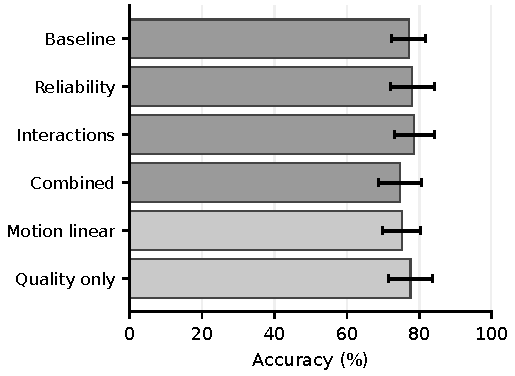
\includegraphics[width=\columnwidth]{figures/pose_results.pdf}
\caption{Corrected CPU crowd accuracy. Error bars summarize descriptive fold/seed variation for TCNs and fold variation for deterministic controls. They are not confidence intervals.}
\label{fig:pose}
\end{figure}

\subsection{Matched centering and coverage changes}
The paired centering study gives interaction accuracy 76.5\% under the legacy origin and 78.6\% under the corrected origin, an increase of 2.18 percentage points calculated from unrounded means. Reliability increases by 0.95 points. Baseline decreases by 0.54 points and combined decreases by 0.27 points (Table~\ref{tab:center}). The unchanged motion and quality controls reproduce the same held-out scores and decisions across the matched CPU studies.

These results support treating origin construction as a material implementation choice. They do not show that every pose model benefits from interpolation or that an interaction improvement transfers externally. Dependent paired runs and descriptive variation do not establish statistical significance. The correction also retains an offline dependence on complete observed segments.

\begin{table}[t]
\caption{Matched CPU centering comparison. Changes use unrounded source values and percentage points (pp).}
\label{tab:center}\centering
\begin{tabular}{lrrr}
\toprule
Variant & Legacy & Corrected & Change\\
\midrule
Baseline & 77.6\% & 77.0\% & -0.54 pp\\
Reliability & 77.1\% & 78.1\% & +0.95 pp\\
Interactions & 76.5\% & 78.6\% & +2.18 pp\\
Combined & 75.0\% & 74.7\% & -0.27 pp\\
\bottomrule
\end{tabular}
\end{table}

The earlier explicit-coverage GPU ablation leaves three variant mean accuracies unchanged and reduces interaction accuracy by 0.14 percentage points. Accuracy ties can contain changed decisions. Other masks and detection-related channels remain available, so the ablation does not remove the predictive quality signal demonstrated by the aggregate control. Its legacy-feature GPU values are retained separately from the matched corrected CPU results.

\subsection{Input controls}
Table~\ref{tab:controls} compares fresh GPU fits of the same corrected combined TCN. Full input reaches 75.4\%, detection-only reaches 72.5\%, and shuffled-time input reaches 75.4\%. Detection-only falls by 2.86 percentage points using unrounded means. It nevertheless retains substantial predictive ability after removal of explicit kinematic channels.

Equal mean accuracy under shuffled time does not imply identical decisions or equal values of all metrics. Its macro-F1 is 0.744 rather than 0.747, and its mean AUC is 0.863 rather than 0.859. More fundamentally, the permutation retains derived velocities within slices. The experiment therefore gives a bounded finding about ordering under this implementation, rather than a conclusion that temporal motion is unnecessary.

\begin{table}[t]
\caption{Matched corrected combined-TCN GPU input controls. Accuracy is mean percent with descriptive standard deviation.}
\label{tab:controls}\centering
\begin{tabular}{lrrr}
\toprule
Condition & Accuracy & F1 & AUC\\
\midrule
Full & 75.4 $\pm$ 4.7 & 0.747 & 0.859\\
Detection only & 72.5 $\pm$ 5.5 & 0.716 & 0.834\\
Shuffled time & 75.4 $\pm$ 6.0 & 0.744 & 0.863\\
\bottomrule
\end{tabular}
\end{table}


\subsection{Frozen crowd video reference}
The frozen R3D-18 reference reaches 91.0\% mean crowd accuracy, macro-F1 0.909, and ROC-AUC 0.979, with descriptive accuracy standard deviation 4.47 percentage points across its five heads. These values exceed the implemented pose variants under the same clip assignments. However, the video encoder has external action pretraining and a different architecture and fitting procedure. We report a strong reference in this setup rather than a causal result that RGB appearance alone explains the difference.

Earlier frozen crowd-video transfer to the 400 RWF evaluation clips gives 63.25\% accuracy for the fixed fold-1 head and 63.75\% for a predeclared equal-weight five-head ensemble. Those heads receive no RWF fitting. An earlier crowd-trained legacy combined pose checkpoint gives 56.0\% RWF transfer accuracy at its original threshold 0.54. That checkpoint differs from the corrected interactions model used externally later. These exploratory transfer results motivated a separate supervised reference; they are not matched adaptation controls for the final fine-tuning experiment.

\subsection{Validation-selected surveillance models}
The supervised frozen RWF reference gives validation accuracy 82.0\%, macro-F1 0.819, and Fight recall 73.6\%. The extra temporal-window candidate gives 81.7\% accuracy, macro-F1 0.816, and validation log loss 0.39543, compared with 0.39298 for the reference. It fixes 12 previous validation errors and introduces 13 new ones. Although Fight misses decrease from 42 to 40, false alarms increase from 15 to 18. It fails the promotion conjunction and remains unevaluated on the released evaluation set.

The layer4 candidate passes all three promotion criteria. At epoch 2, validation log loss is 0.33700, macro-F1 is 0.864, and Fight recall is 91.8\%. Accuracy is 86.4\%, with 13 missed fights and 30 false alarms. Table~\ref{tab:validation} summarizes the chosen operating point. Fig.~\ref{fig:loss} shows the recorded validation losses across all eight epochs. Selection follows minimum log loss, not the highest accuracy observed at another epoch. The chosen checkpoint and threshold remain fixed in the following evaluations.

\begin{table}[t]
\caption{RWF validation comparison on 317 clips. The chosen fine-tuned checkpoint is epoch 2.}
\label{tab:validation}\centering
\begin{tabular}{lrr}
\toprule
Metric & Frozen & Fine-tuned\\
\midrule
Log loss & 0.393 & 0.337\\
Accuracy & 82.0\% & 86.4\%\\
Macro-F1 & 0.819 & 0.864\\
Fight recall & 73.6\% & 91.8\%\\
Threshold & 0.50 & 0.23\\
\bottomrule
\end{tabular}
\end{table}

\begin{figure}[t]
\centering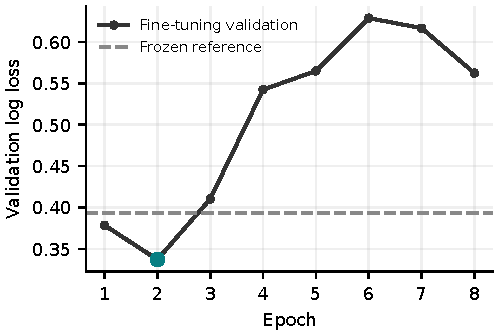
\includegraphics[width=\columnwidth]{figures/validation_loss.pdf}
\caption{Recorded validation log loss across the bounded fine-tuning run. The highlighted epoch 2 has the minimum loss. The dashed line is the original frozen reference.}
\label{fig:loss}
\end{figure}

\subsection{Fixed RWF evaluation}
Table~\ref{tab:evaluation} and Fig.~\ref{fig:rwfcm} compare both video models on all 400 RWF evaluation clips. Frozen accuracy is 84.0\% and fine-tuned accuracy 83.75\%. Fine-tuning increases Fight recall from 78.5\% to 87.5\% and AUC from 0.900 to 0.929. It reduces misses from 43 to 25 but increases false alarms from 21 to 40. With 200 clips per class, the false-positive rate changes from 10.5\% to 20.0\%, and the missed-Fight rate changes from 21.5\% to 12.5\%.

The selected candidate therefore exchanges 18 fewer misses for 19 more false alarms. Macro-F1 changes from 0.840 to 0.837, and violent precision decreases from 88.2\% to 81.4\%. Improved score ranking and recall do not require improved thresholded accuracy. Because thresholds are 0.50 and 0.23, the comparison combines parameter adaptation with a changed operating point. No additional threshold is tuned on these results.

\begin{table*}[t]
\caption{Fixed all-clip evaluation. Fight is positive. FP counts nonviolent clips flagged violent, and FN counts missed violent clips.}
\label{tab:evaluation}\centering
\begin{tabular}{llrrrrrrrrr}
\toprule
Set & Model & $n$ & $\tau$ & Accuracy & F1 & AUC & Precision & Recall & FP & FN\\
\midrule
RWF & Frozen video & 400 & 0.50 & 84.00\% & 0.840 & 0.900 & 88.2\% & 78.5\% & 21 & 43\\
RWF & Fine-tuned video & 400 & 0.23 & 83.75\% & 0.837 & 0.929 & 81.4\% & 87.5\% & 40 & 25\\
Hockey & Frozen video & 1000 & 0.50 & 70.80\% & 0.686 & 0.886 & 94.1\% & 44.4\% & 14 & 278\\
Hockey & Fine-tuned video & 1000 & 0.23 & 81.10\% & 0.810 & 0.893 & 86.6\% & 73.6\% & 57 & 132\\
Hockey & Crowd pose & 1000 & 0.62 & 40.90\% & 0.361 & 0.420 & 44.1\% & 68.2\% & 432 & 159\\
\bottomrule
\end{tabular}
\par\smallskip\parbox{\textwidth}{\footnotesize RWF results use previously inspected footage. All 1,000 Hockey mirror clips remain. The frozen video reference is the predeclared primary external model; fine-tuning is supplementary and crowd pose is diagnostic.}
\end{table*}

\begin{figure*}[t]
\centering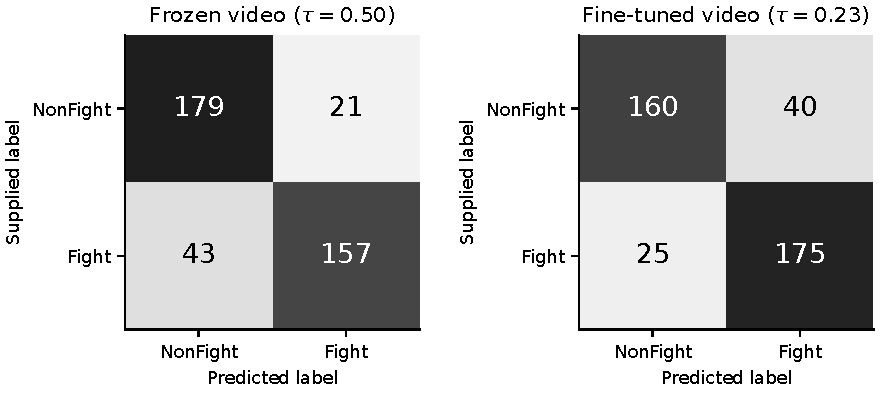
\includegraphics[width=.86\textwidth]{figures/rwf_confusion.pdf}
\caption{RWF all-clip confusion counts. Rows use supplied labels and columns use predictions. Fine-tuning at its validation-selected threshold reduces missed fights but increases false alarms.}
\label{fig:rwfcm}
\end{figure*}

\subsection{External hockey evaluation}
The fixed frozen RWF video model reaches 70.8\% accuracy on all 1,000 hockey clips. Its precision is 94.1\% but Fight recall only 44.4\%, with 278 misses and 14 false alarms. The supplementary fine-tuned model reaches 81.1\% accuracy and 73.6\% recall, with 132 misses and 57 false alarms. Its AUC is 0.893, compared with 0.886 for frozen video. Fig.~\ref{fig:external} illustrates the accuracy and recall differences.

The corrected crowd interactions checkpoint reaches 40.9\% accuracy, macro-F1 0.361, and AUC 0.420. It flags 432 of 500 nonviolent clips, while detecting 341 of 500 violent clips. Restricting to the 982 pose-supported clips gives 40.63\% accuracy and does not rescue performance. Poor support is therefore insufficient to explain the external failure. Sports-domain geometry, tracking behavior, threshold transfer, and missing context remain possible contributors, without a causal attribution from this experiment.

\begin{figure}[t]
\centering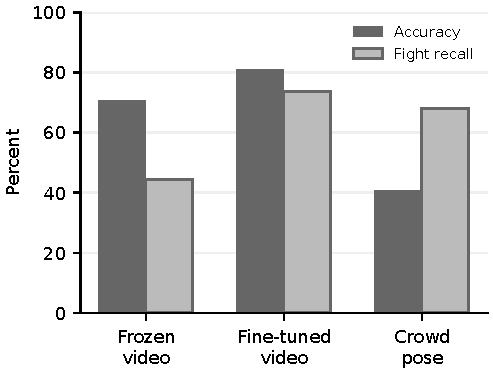
\includegraphics[width=\columnwidth]{figures/external_results.pdf}
\caption{All-clip Hockey Fight accuracy and Fight recall for fixed models. The video models were fitted on RWF, while the pose checkpoint was fitted on crowd footage.}
\label{fig:external}
\end{figure}

\subsection{Diagnostic clips and measured runtime}
Four final video examples cover true-positive, true-negative, false-positive, and false-negative outcomes relative to supplied labels. They are the most confident available examples in their confusion categories, selected after scoring for explanation. Each saved five-second MP4 contains 150 frames, fully decodes, and reproduces its stored score with zero observed drift. This verifies the saved demonstration and is not an independent accuracy sample.

Fig.~\ref{fig:failures} shows two error examples. The false-positive score is 0.999659 and the false-negative score 0.004315 at threshold 0.23. Neither the extremity of a score nor the appearance of one frame establishes correct labeling or explains the failure mechanism. These scores also show why the classifier output should not be presented as calibrated incident probability.

\begin{figure*}[t]
\centering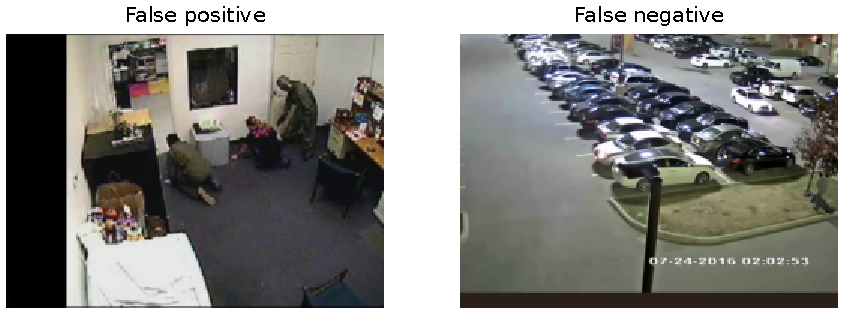
\includegraphics[width=.94\textwidth]{figures/failure_examples.pdf}
\caption{Frames cropped from saved RWF diagnostic videos. Left: supplied nonviolent label, violent prediction, score 0.999659. Right: supplied violent label, nonviolent prediction, score 0.004315. These outcome-selected examples illustrate disagreement with unreviewed supplied labels, not independently verified ground truth.}
\label{fig:failures}
\end{figure*}

Table~\ref{tab:runtime} gives warm pose-pipeline median 0.270 s and p95 0.390 s. Cold external-process median is 8.359 s and p95 8.503 s. Warm median pose/tracking time is 0.2408 s, whereas classifier time is 0.00246 s, illustrating why model-only timing would misrepresent the full pipeline. Component medians need not sum to the median of total time. Fig.~\ref{fig:runtime} shows individual recorded measurements with separate units for warm and cold boundaries.

The eight-epoch fine-tuning run takes 327.32 s and records peak PyTorch allocated GPU memory of 621,134,848 bytes, approximately 0.62 GB in decimal units. This is an allocator measurement, not total device memory. These training and pose-inference measurements do not establish fine-tuned RGB streaming speed or throughput.

\begin{table}[t]
\caption{Offline pose timing on ten fixed clips. Overlay generation and export are excluded.}
\label{tab:runtime}\centering
\begin{tabular}{lrr}
\toprule
Measurement & Median (s) & p95 (s)\\
\midrule
Warm pipeline (30 runs) & 0.270 & 0.390\\
Cold external process (10) & 8.359 & 8.503\\
\bottomrule
\end{tabular}
\end{table}

\begin{figure*}[t]
\centering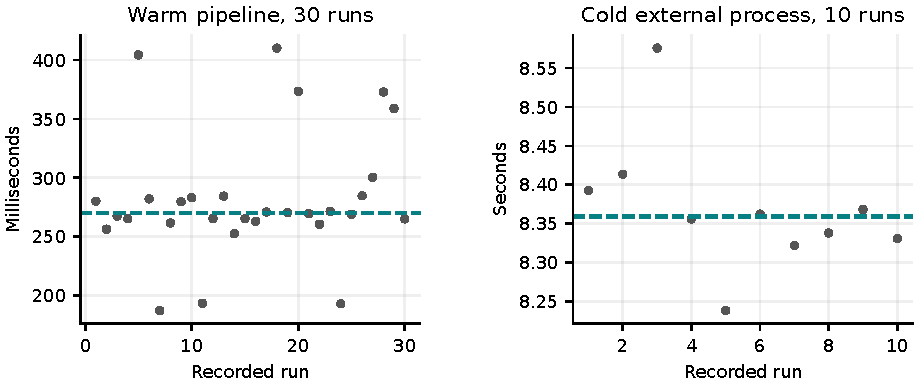
\includegraphics[width=.93\textwidth]{figures/runtime_runs.pdf}
\caption{Recorded pose timing. Warm values include the pipeline with loaded models; cold values include an external Python process and initialization. Axes use different units and scales. Dashed lines show medians. Overlay/export is excluded.}
\label{fig:runtime}
\end{figure*}

\section{Discussion and Limitations}
\subsection{What the pose experiments establish}
The corrected crowd study gives a modest mean accuracy advantage to interactions and reliability relative to the baseline, with no combined gain. This outcome does not establish a universal benefit or a failure of interaction modeling in general. The nearest-person features may be useful in some recordings and noisy in others. Added confidence channels can provide information while increasing parameter count and exposing estimator behavior. The current experiment does not isolate which of these possibilities drives the combined result.

Centering changes matter because derived velocities depend on the coordinate origin. The matched CPU comparison isolates that construction choice more carefully than comparing historical GPU fitting with a corrected CPU run. Its mixed variant results are a reason to record preprocessing precisely. A stable origin does not repair all missing joints, wrong associations, or camera motion, and complete-segment interpolation prevents a direct causal streaming interpretation.

The detection controls also require precise language. Competitive quality-only performance demonstrates predictive aggregate cues. Detection-only TCN performance shows that retained per-frame quality and presence information remains useful after zeroing selected kinematics. Neither proves that every full-model decision depends on a shortcut or identifies a specific scene bias. The unchanged explicit-coverage means cannot eliminate this concern because indirect cues remain. The ordering control retains precomputed velocity and therefore cannot support the statement that motion is irrelevant.

\subsection{Interpreting the video comparison}
The frozen crowd video reference provides a stronger result under the same clip assignments, but it has substantial action pretraining and different model capacity. Pretraining-source overlap is unaudited. Its result motivates a practical reference and further testing, rather than a conclusion that pose features are inherently inferior across datasets, architectures, or tasks.

The supervised RWF reference changes the downstream training domain. The later fine-tuning comparison is within that domain and follows an explicit validation rule. Its higher AUC and Fight recall accompany lower precision and slightly lower accuracy on RWF. The hockey result improves both accuracy and recall but still has 132 missed fights and 57 false alarms. Thus improved external accuracy does not mean every relevant operating requirement is met.

A lower selected threshold can account for part of the recall/false-alarm shift. Separating the effect of adapted weights from operating-point selection would require additional matched-threshold or fixed-cost analyses declared independently of the completed evaluations. We do not retroactively tune the current threshold to obtain a more favorable comparison. A deployment setting would also need a justified balance between missed incidents and unnecessary review; macro-F1 on development clips is not itself that application policy.

\subsection{Data exposure and uncertainty}
The crowd and RWF footage had been inspected before the final studies. Source grouping and later sealing improve internal separation, but they do not restore an untouched test. Known source merges and duplicate exclusions address identified overlap, while unknown reused footage and Kinetics overlap remain possible. Hockey's byte comparison rules out byte-identical files against the declared inventory but does not establish independent games or complete near-duplicate separation.

Labels remain supplied and independently unreviewed. A high-confidence false positive could reflect classifier failure, label ambiguity, or both; a selected frame cannot distinguish those explanations. A future independent review should assess full clips under a documented rubric before inspecting model scores. That process should preserve the current results and record any revised-label experiment separately rather than silently changing the completed evaluation.

Fold/seed variation is descriptive. Repeated clips, shared training sets, and known source dependence invalidate an interpretation of all repeated decisions as independent observations. The manuscript therefore reports no significance claim from small mean differences. The fine-tuning result also comes from one bounded seed-42 run. It does not establish robustness over fine-tuning seeds, hardware, or hyperparameter budgets.

\subsection{Scope, privacy, and operational behavior}
All primary outputs concern complete short clips. Uniform sparse sampling can miss short events, average pooling can lose temporal position, and masked person pooling can lose individual attribution. A closed-window interface can process longer videos offline, but window accounting alone does not validate outbreak detection, continuous-stream false-alarm rates, or latency under live load. The pose benchmark covers ten fixed clips and one laptop GPU, with export excluded.

Pose representation can omit some raw appearance from classifier input, yet the pipeline still processes videos and can expose contextual or identifying motion. It implements no formal privacy guarantee, federated system, or security audit. Neither tracks nor clip scores establish responsibility, intent, or individual guilt. Any operational proposal would require additional reviewed data, domain-specific validation, error-cost analysis, and handling of uncertain or ambiguous clips.

The next research step is a fresh, independently reviewed evaluation corpus with more complete recording-source information. Predeclared analyses could examine fixed operating points, stability over seeds, actual occlusion and association failures, and temporal-event coverage. Those are future experiments. The current archive supplies reproducible evidence of implemented behavior and its limitations, including negative findings, rather than substituting computational checks for independent evaluation.

\section{Conclusion}
This study evaluates pose reliability and nearest-person interactions under a controlled crowd-classification implementation and adds separate pretrained video references and bounded RWF fine-tuning. Corrected interactions reach 78.6\% mean crowd accuracy, but combined features do not improve the baseline. Quality and detection controls remain predictive, and time shuffling retains motion within derived slices. Frozen video features give a stronger crowd reference. Validation-selected fine-tuning improves Fight recall and supplementary hockey accuracy, while increasing RWF false alarms and slightly reducing accuracy. Poor crowd-pose transfer further limits generalization claims. Source exposure, incomplete overlap audits, dependent repeated observations, and pending independent labels keep the findings exploratory. The released implementation and saved records support reproducible follow-up work on offline clip classification.

\appendices
\section{Implementation and Evidence Records}
\subsection{Experiment identities}
The project archive distinguishes experiments by dated directories and frozen protocol hashes. The primary pose results use the corrected CPU experiment and its matched legacy CPU reference. The GPU input controls and earlier coverage ablation are separate experiments, preserving device and feature-schema differences. The accompanying experiment index maps each manuscript study to its exact archive directory and principal result files.

Separate records identify the crowd video heads, crowd-head RWF transfer, supervised frozen RWF head, rejected temporal candidate, and retained layer4 checkpoint. The fine-tuning record includes validation promotion and all eight training epochs. Final RWF and external Hockey scores each have their own fixed evaluation record. This separation prevents mixing validation, evaluation, and historical transfer results.

An accompanying evidence manifest records hashes of the source result files used to generate manuscript tables and figures. The figures use saved metrics, histories, timings, and posters rather than newly fitted scores. Rounded display values do not replace full-precision source records. Confusion counts and all-clip denominators are checked when generating tables, and the fitting/evaluation archive is read without modification.

\subsection{Checkpoints, input support, and numeric reproduction}
The corrected pose transfer checkpoint is fold 1, seed 42, interactions, threshold 0.62. Its SHA-256 prefix is \texttt{11cf6c9ca0b5b229}. The fine-tuned checkpoint prefix is \texttt{04692366a21cd546}, and the frozen RWF logistic-model prefix is \texttt{50283bc44a38c604}. The accompanying evidence manifest records the full hashes. They identify the exact saved artifacts, not their scientific validity.

Raw pose caches preserve normalized joints, boxes, observation masks, frame indices, timestamps, track IDs, source hashes, and extraction signatures. Derived corrected features are recomputed from those caches. The raw pose extraction descriptor retains its archived schema label while each classifier records the derived feature schema explicitly. Old checkpoints use their recorded legacy semantics rather than receiving an undocumented correction at inference.

The bounded video decoder reproduces uniform sampling using the actual decoded frame count and retains only selected frames for whole-clip inference. The longer-video interface processes nonoverlapping closed windows offline and records a single-frame tail without assigning it a model prediction. Implementation tests check these accounting behaviors; they do not quantify missed event coverage between samples.

CUDA numeric reproduction can depend on batch shape. The final single-video path preserves the recorded validation batch shape to match the saved score rounding. Fine-tuned scores are not calibrated probabilities. Pose-supported status derives from the recorded valid-joint rule, with a pre-existing 25\% usable-sampled-frame cutoff for the diagnostic subset. Primary evaluation still includes all clips. A support flag is not a validated rejection policy.

\subsection{Runtime environment and sharing}
The recorded final environment uses Python 3.13, PyTorch 2.11.0 with CUDA 12.8, TorchVision 0.26.0, NumPy 2.5.2, OpenCV 4.14.0.94, and scikit-learn 1.9.1. The experiment-specific protocols preserve package versions and implementation hashes. New fitting on another environment requires a new named experiment, rather than rewriting a sealed record. CPU and GPU numerical checks have separately recorded tolerances and outcomes.

Code, selected evidence, the small pose checkpoint, logistic parameters, and final RGB diagnostic videos are available through the project repository \cite{projectrepo}. Raw datasets, pretrained weights, caches, local environments, and the large fine-tuned checkpoint are separate assets. Some historical report links and hashes therefore refer to files in the full local archive rather than a minimal clone. The repository setup guide describes required weights and expected hashes.

Saved pose demonstrations use the corrected interactions checkpoint and sampled skeleton overlays. Final RGB demonstrations use the fine-tuned checkpoint and show a whole-clip decision. These two sets illustrate different models and should not be interchanged when explaining feature use. All outcome-selected demonstrations are diagnostic examples rather than independent performance samples. The independent review pack remains neutral and incomplete, and its coordinator mapping is kept outside the shared repository.

% Balance the final reference columns in this review copy; revisit after edits.
\IEEEtriggeratref{10}
\bibliographystyle{IEEEtran}
\bibliography{references}
\end{document}
